\section{Darkroom. Alternative Split}
\label{appendix:gridworld_alternative_split}
A random split of actions in Darkroom environment may lead to a data leakage as multiple action sequences result in  the same endpoint. To address this, we conducted an experiment with distinct, non-overlapping action sets for training and testing. We trained Headless-AD with actions that cause movements of $0$, $1$, and $3$ cells, and tested on movements of $2$ cells, introducing scenarios not encountered during training.

\Cref{fig:split_3_gridworld_bars} shows that although Headless-AD experienced a slight decrease in performance on the test action set, it still remained significantly above the random level and outreaching the AD-level, underscoring its capability to generalize beyond the training action space. This experiment intends to make the capabilities and limitations of Headless-AD clearer.


\begin{figure*}[t]
    \vskip 0.2in
    \centering
    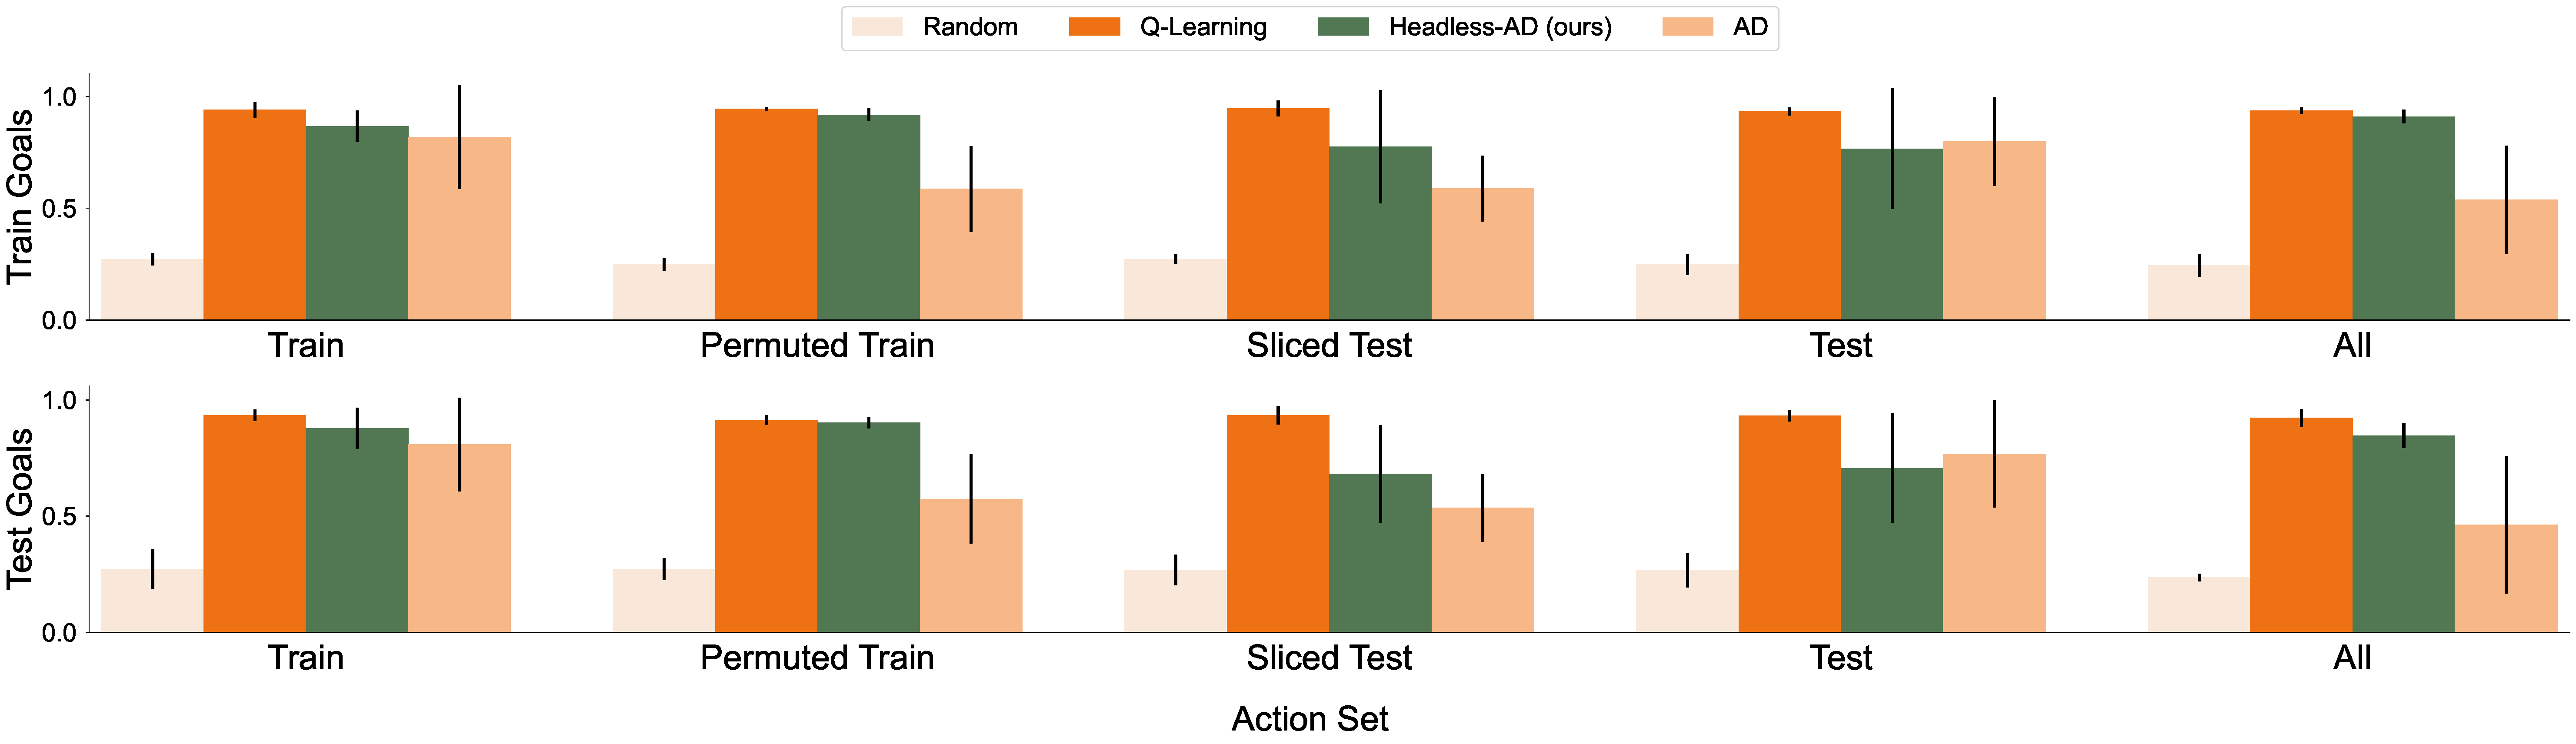
\includegraphics[width=0.9\textwidth]{images/split_3_gridworld_bars.pdf}
    \caption{\textbf{Darkroom. Alternative Split:} In this experiment the actions in Darkroom were split into non-overlapping in terms of the distance of the endpoint from the initial position. Train split consisted of actions with length $0$, $1$ and $3$, test split - $2$. Headless-AD, though with a slight drop, maintained its performance on levels seen during the previous experiment with a random split.}
    \label{fig:split_3_gridworld_bars}
    \vskip -0.2in
\end{figure*}